\documentclass[11pt,a4paper]{ctexart}

\usepackage{amsmath,amssymb,amsthm,mathtools}
\usepackage{booktabs,tabularx,longtable,multirow}
\usepackage{graphicx,float}
\usepackage{xcolor}
\usepackage{geometry}
\usepackage{hyperref}
\usepackage{enumitem}
\usepackage{algorithm}
\usepackage{algpseudocode}
\usepackage[most]{tcolorbox}
\usepackage{listings}

\geometry{left=2.15cm,right=2.15cm,top=2.25cm,bottom=2.25cm}
\graphicspath{{../results/figures/}}
\hypersetup{
  colorlinks=true,
  linkcolor=blue!55!black,
  citecolor=blue!55!black,
  urlcolor=blue!55!black
}
\setlength{\parindent}{2em}
\setlength{\parskip}{0.2em}
\setlist[itemize]{leftmargin=2em}
\setlist[enumerate]{leftmargin=2.4em}

\definecolor{DeepBlue}{HTML}{1F4E79}
\definecolor{LightBlue}{HTML}{EEF5FB}
\definecolor{DeepGreen}{HTML}{2F6B4F}
\definecolor{LightGreen}{HTML}{EFF8F2}
\definecolor{DeepOrange}{HTML}{9A4E00}
\definecolor{LightOrange}{HTML}{FFF5E8}
\definecolor{SoftGray}{HTML}{F4F5F7}

\newtcolorbox{conceptbox}[1]{
  enhanced,
  breakable,
  colback=LightBlue,
  colframe=DeepBlue,
  fonttitle=\bfseries,
  title={#1},
  boxrule=0.7pt,
  arc=1.5mm
}
\newtcolorbox{resultbox}[1]{
  enhanced,
  breakable,
  colback=LightGreen,
  colframe=DeepGreen,
  fonttitle=\bfseries,
  title={#1},
  boxrule=0.7pt,
  arc=1.5mm
}
\newtcolorbox{boundarybox}[1]{
  enhanced,
  breakable,
  colback=LightOrange,
  colframe=DeepOrange,
  fonttitle=\bfseries,
  title={#1},
  boxrule=0.7pt,
  arc=1.5mm
}

\newtheorem{proposition}{命题}[section]
\newtheorem{definition}[proposition]{定义}
\newcommand{\E}{\mathbb E}
\newcommand{\Qset}{\mathcal Q}
\newcommand{\Types}{\Theta}
\newcommand{\Priors}{\mathcal M}
\newcommand{\Costs}{\mathcal C}
\newcommand{\Grid}{\mathcal G}
\newcommand{\Rev}{\operatorname{Rev}}
\newcommand{\ind}{\mathbb I}

\algrenewcommand\algorithmicrequire{\textbf{输入：}}
\algrenewcommand\algorithmicensure{\textbf{输出：}}
\floatname{algorithm}{算法}

\lstset{
  basicstyle=\ttfamily\small,
  backgroundcolor=\color{SoftGray},
  frame=single,
  breaklines=true,
  columns=fullflexible
}

\title{\textbf{数据增强型 AutoML 市场的机制改进}\\
\large 概念解读、数学模型、伪代码与实验验证}
\author{基于《Optimal Pricing for Data-Augmented AutoML Marketplaces》的课程项目扩展}
\date{2026年7月24日\quad 版本 0.7.1}

\begin{document}
\maketitle

\begin{abstract}
原论文把数据增强、AutoML 模型发现、买家最优停止与性能提升定价连接成一个统一市场。其核心思想是：平台不按数据表数量或训练计算量收费，而是对最终可测的模型性能提升发布价格曲线。该框架具有清晰的经济含义，但从复现走向部署时仍有四个关键边界：论文式定价实验采用强制购买口径；平台在冷启动阶段并不知道真实买家先验；非零搜索成本会改变买家的停止行为；数据发现过程与后续收入目标相互割裂。

本文详细说明项目在不改变“按性能提升定价”主线的前提下所做的四项改进：加入不购买外部选项；用精确状态传播实现成本感知 Markov 定价；在多个先验与搜索成本场景上做有限场景 max--min 鲁棒优化；用 warm-start 价格信号引导 Data-Bandit。报告给出概念解释、目标函数、动态规划、状态传播、四段伪代码、复杂度、实验设置、主实例与多实例结果、价格信号消融以及适用边界。实验表明，Cost-aware Markov 在名义市场中收入最高，Robust cost-aware Markov 提高最坏情况收入，而 Pricing-guided Data-Bandit 能更早发现高价值增强；这些收益均伴随明确的假设和权衡。
\end{abstract}

\tableofcontents
\newpage

\section{阅读目标与改进总览}

这份报告回答三个问题：

\begin{enumerate}
  \item 原论文模型的部署边界究竟是什么，为什么不能只改实验口径而不改买家响应？
  \item 每项改进修改了哪个数学对象：可选集合、动态收入、优化目标，还是发现算法？
  \item 实验数字能支持多强的结论，哪些结果不能外推为一般理论？
\end{enumerate}

\begin{table}[H]
\centering
\small
\caption{四项改进与原模型边界的对应关系。}
\begin{tabularx}{\textwidth}{p{2.7cm}p{3.0cm}X p{2.7cm}}
\toprule
改进 & 原模型边界 & 修改的核心对象 & 主要验证指标\\
\midrule
外部选项 / IR-aware &
强制每个买家购买 &
买家可选集合加入零效用、零支付选项 &
自愿购买实现收入\\
\addlinespace
成本感知 Markov &
$c\approx0$ 时把轨迹压缩为集合 &
价格、停止策略、Markov 顺序联合进入收入 &
精确动态收入\\
\addlinespace
有限场景鲁棒定价 &
买家先验和搜索成本被视为已知 &
最大化多个先验/成本场景中的最坏收入 &
最坏场景收入\\
\addlinespace
价格引导 Data-Bandit &
发现与定价分成独立模块 &
访问顺序与 bandit 奖励加入 warm-start 收入信号 &
AUC、早期效用\\
\bottomrule
\end{tabularx}
\end{table}

\begin{conceptbox}{一句话理解}
四项改进不是把市场改回“按数据量收费”，而是在同一条性能提升价格曲线 $x(q)$ 上依次修正“可以买不买”“何时停止”“先验不确定”和“先发现什么”四个问题。
\end{conceptbox}

\section{原论文模型：改进从哪里开始}

\subsection{质量、买家类型与价格曲线}

设离散质量空间为 $\Qset=\{1,\ldots,Q\}$，买家类型集合为
$\Types=\{1,\ldots,K\}$。类型 $\theta$ 对质量 $q$ 的估值为
$v^\theta(q)$，平台公布价格曲线 $x(q)\ge0$。买家从质量 $q$ 得到的净价值为
\[
u^\theta(q;x)=v^\theta(q)-x(q).
\]

AutoML 发现过程产生随机质量序列
$Q_1,Q_2,\ldots,Q_T$。初始状态服从 $\rho$，转移概率为
\[
P_t(q'\mid q)=\Pr(Q_{t+1}=q'\mid Q_t=q).
\]
平台不直接出售某张外部数据表，而是出售发现过程最终带来的可测质量或性能提升。

\subsection{论文式样本平均定价}

当每轮搜索成本近似为零时，一条轨迹的到达顺序不再重要，可以压缩为出现过的质量集合 $s\subseteq\Qset$。论文式 forced-choice 响应为
\[
q_{\theta,s}^{\mathrm{FC}}(x)
\in\arg\max_{q\in s}\{v^\theta(q)-x(q)\}.
\]
给定 $m$ 个样本集合 $s_1,\ldots,s_m$ 和类型先验 $\mu$，经验收入为
\[
\widehat{\Rev}_{\mathrm{FC}}(x;\mu)
=\sum_{\theta\in\Types}\mu_\theta
  \frac1m\sum_{j=1}^{m}x\!\left(q_{\theta,s_j}^{\mathrm{FC}}(x)\right).
\]

该目标适合复现论文的定价 MILP，但它隐含一个强假设：即使所有质量的净效用都为负，买家仍必须选一个质量并付款。这是第一项改进的起点。

\subsection{四个部署边界}

\begin{enumerate}
  \item \textbf{购买语义：}真实买家可以退出；forced-choice 收入可能记录经济上无法实现的支付。
  \item \textbf{顺序与成本：}当 $c>0$ 时，晚出现的高质量未必能被买家等到；相同到达集合可能产生不同收入。
  \item \textbf{参数不确定：}最优价格依赖类型先验 $\mu$ 和搜索成本 $c$，而冷启动时两者都可能估计不准。
  \item \textbf{发现目标：}普通 Data-Bandit 追求尽快发现高验证效用组合，但平台最终关心的还包括可实现收入。
\end{enumerate}

\section{改进一：外部选项与自愿购买语义}

\subsection{概念解读}

外部选项表示“什么也不买”。记该选项为 $\varnothing$，规定
\[
v^\theta(\varnothing)=0,\qquad x(\varnothing)=0,\qquad
u^\theta(\varnothing;x)=0.
\]
于是买家的真实选择变为
\[
q_{\theta,s}^{\mathrm{IR}}(x)
\in\arg\max_{q\in s\cup\{\varnothing\}}
\{v^\theta(q)-x(q)\}.
\]
相应的经验实现收入为
\[
\widehat{\Rev}_{\mathrm{IR}}(x;\mu)
=\sum_{\theta\in\Types}\mu_\theta\frac1m\sum_{j=1}^{m}
x\!\left(q_{\theta,s_j}^{\mathrm{IR}}(x)\right),
\]
其中 $x(\varnothing)=0$。

\begin{conceptbox}{为什么称为“语义修正”}
外部选项并不是一个新的收费规则。平台仍对性能提升质量 $q$ 定价；变化只在于买家不会在所有净效用为负时被迫购买。因此 IR-aware 的首要作用是让评价指标与可退出市场一致，而不是保证收入必然超过所有基线。
\end{conceptbox}

\begin{proposition}[个体理性]
在外部选项下，买家的购买前净效用满足
\[
\max_{q\in s\cup\{\varnothing\}}u^\theta(q;x)\ge0.
\]
因此买家不会被分配到严格负净效用的质量。
\end{proposition}

\begin{algorithm}[H]
\caption{带外部选项的买家响应与支付}
\begin{algorithmic}[1]
\Require 可达质量集合 $s$，估值 $v^\theta$，价格曲线 $x$
\Ensure 所选质量 $q^\star$ 与平台支付 $p$
\State $q^\star\gets\varnothing$，$U^\star\gets0$，$p\gets0$
\For{$q\in s$}
  \State $U\gets v^\theta(q)-x(q)$
  \If{$U>U^\star$，或 $U=U^\star$ 且 $x(q)>p$}
    \State $q^\star\gets q$，$U^\star\gets U$，$p\gets x(q)$
  \EndIf
\EndFor
\State \Return $(q^\star,p)$
\end{algorithmic}
\end{algorithm}

实现使用卖方有利的效用平局处理：若买家在零效用购买与退出之间无差异，可以选择价格更高的同效用质量。报告结果因此应理解为声明过的平局规则下的收入，而不是所有平局规则下的下界。

\section{改进二：成本感知的精确 Markov 定价}

\subsection{为什么集合压缩在 \texorpdfstring{$c>0$}{c > 0} 时失效}

考虑两条轨迹 $(q_L,q_H)$ 与 $(q_H,q_L)$。二者可达集合相同，但如果继续搜索需要支付成本，第一条轨迹中的买家可能在 $q_L$ 就停止，而第二条轨迹一开始便能购买 $q_H$。因此收入不仅取决于“见过哪些质量”，还取决于出现顺序、剩余时域和转移概率。

\begin{proposition}[价格--停止耦合]
当搜索成本 $c>0$ 时，一般不存在只依赖最终可达集合 $s$ 的收入函数，能够对所有到达顺序准确表示平台收入。
\end{proposition}

\subsection{最优停止动态规划}

对类型 $\theta$，令 $b$ 表示历史上净价值最高的质量，$q$ 表示当前质量。若下一轮出现 $q'$，历史最佳状态更新为
\[
B^\theta_x(b,q')=
\begin{cases}
b,&u^\theta(b;x)\ge u^\theta(q';x),\\
q',&u^\theta(q';x)>u^\theta(b;x).
\end{cases}
\]

第 $t$ 轮停止时，前 $t$ 轮搜索成本已经发生。允许退出时的停止价值为
\[
S_t^\theta(b;x,c)=\max\{u^\theta(b;x),0\}-ct.
\]
终点必须停止：
\[
V_T^\theta(b,q)=S_T^\theta(b;x,c).
\]
对 $t<T$，Bellman 递推为
\[
V_t^\theta(b,q)=
\max\left\{
S_t^\theta(b;x,c),\
\sum_{q'\in\Qset}P_t(q'\mid q)
V_{t+1}^\theta(B^\theta_x(b,q'),q')
\right\}.
\]
若右侧继续价值严格大于停止价值，则策略
$\pi_t^\theta(b,q;x,c)=1$，否则停止。

\subsection{精确状态前向传播}

只求出停止策略还不等于求出收入。项目进一步传播状态概率，而不是采样有限条轨迹。令
\[
\alpha_t^\theta(b,q)=
\Pr(\text{第 }t\text{ 轮仍活跃且状态为 }(b,q)\mid\theta).
\]
初始概率为
\[
\alpha_1^\theta(b,q)=\rho(q)\ind\{b=q\}.
\]
若状态继续，则
\[
\alpha_{t+1}^\theta(b',q')
\mathrel{+}=
\alpha_t^\theta(b,q)P_t(q'\mid q),
\qquad b'=B^\theta_x(b,q').
\]
精确类型收入为
\[
\Rev_\theta(x;c)=
\sum_{t=1}^{T}\sum_{b,q}
\alpha_t^\theta(b,q)
\ind\{\text{在 }(t,b,q)\text{ 停止}\}
x(b)\ind\{u^\theta(b;x)\ge0\}.
\]
市场总收入为
\[
\Rev(x;\mu,c)=\sum_{\theta\in\Types}\mu_\theta\Rev_\theta(x;c).
\]

\begin{algorithm}[H]
\caption{给定价格下的精确 Markov 期望支付}
\begin{algorithmic}[1]
\Require $x,v^\theta,\rho,P_{1:T-1},T,c$，是否允许退出
\Ensure 类型 $\theta$ 的精确期望支付 $R_\theta$
\State 用 Bellman 递推求继续策略 $\pi^\theta$
\State 初始化 $\alpha(b,q)\gets\rho(q)\ind\{b=q\}$，$R_\theta\gets0$
\For{$t=1,\ldots,T$}
  \State 初始化下一轮概率 $\alpha^+(b,q)\gets0$
  \ForAll{$(b,q)$ 且 $\alpha(b,q)>0$}
    \If{$t=T$ 或策略要求停止}
      \If{强制购买，或 $v^\theta(b)-x(b)\ge0$}
        \State $R_\theta\gets R_\theta+\alpha(b,q)x(b)$
      \EndIf
    \Else
      \ForAll{$q'$ 且 $P_t(q'\mid q)>0$}
        \State $b'\gets B^\theta_x(b,q')$
        \State $\alpha^+(b',q')\gets\alpha^+(b',q')+\alpha(b,q)P_t(q'\mid q)$
      \EndFor
    \EndIf
  \EndFor
  \State $\alpha\gets\alpha^+$
\EndFor
\State \Return $R_\theta$
\end{algorithmic}
\end{algorithm}

\subsection{成本感知价格优化}

对每个质量给定有限候选价格集合 $\Grid_q$，价格网格为
$\Grid=\prod_{q\in\Qset}\Grid_q$。名义成本感知价格为
\[
x_{\mathrm{CA}}^\star
\in\arg\max_{x\in\Grid}\Rev(x;\mu,c_0).
\]

这里的“精确”指：\emph{对给定价格、有限状态 Markov 环境和声明的时域，收入通过状态传播精确计算}。价格优化仍限制在有限网格 $\Grid$ 上，因此不宣称是一般连续价格空间中的全局最优解。

\section{改进三：有限场景鲁棒定价}

\subsection{冷启动与分布偏移}

平台的价格依赖买家类型先验 $\mu$，但真实先验通常要通过多轮交易学习。若直接把早期估计当成真值，价格会对冷启动误差和用户结构变化十分敏感。项目用一组可解释场景代替单一估计：
\[
\Priors=\{\mu^{(1)},\ldots,\mu^{(L)}\},\qquad
\Costs=\{c^{(1)},\ldots,c^{(J)}\}.
\]
本实验包括训练先验、OOS 低估值偏移先验、均匀冷启动先验和高估值偏移先验。搜索成本场景为
\[
c\in\{0,0.03,0.08\}.
\]

\subsection{静态 Robust IR 与动态联合鲁棒目标}

静态 Robust IR 在样本集合收入上求
\[
x_{\mathrm{RIR}}^\star
\in\arg\max_{x\in\Grid}
\min_{\mu\in\Priors}
\widehat{\Rev}_{\mathrm{IR}}(x;\mu).
\]

动态 Robust cost-aware Markov 则求
\[
x_{\mathrm{RCA}}^\star
\in\arg\max_{x\in\Grid}
\min_{\mu\in\Priors,\ c\in\Costs}
\Rev(x;\mu,c).
\]

\begin{conceptbox}{鲁棒性意味着什么}
鲁棒目标不是追求每个场景都最好，而是提高最差场景的收入下界。它通常会牺牲名义场景收入，因此适合先验不可靠、搜索成本波动大或平台更重视保守保障的情形。
\end{conceptbox}

\begin{algorithm}[H]
\caption{有限场景鲁棒成本感知定价}
\begin{algorithmic}[1]
\Require 价格网格 $\Grid$，估值矩阵 $V$，先验场景 $\Priors$，成本场景 $\Costs$，Markov 环境
\Ensure 鲁棒价格 $x^\star$ 与最坏场景收入 $z^\star$
\State $z^\star\gets-\infty$
\ForAll{$x\in\Grid$}
  \State $z(x)\gets+\infty$
  \ForAll{$c\in\Costs$}
    \ForAll{$\theta\in\Types$}
      \State 用算法 2 计算 $R_\theta(x;c)$
    \EndFor
    \ForAll{$\mu\in\Priors$}
      \State $z(x)\gets\min\{z(x),\sum_\theta\mu_\theta R_\theta(x;c)\}$
    \EndFor
  \EndFor
  \If{$z(x)>z^\star$}
    \State $(x^\star,z^\star)\gets(x,z(x))$
  \EndIf
\EndFor
\State \Return $(x^\star,z^\star)$
\end{algorithmic}
\end{algorithm}

\begin{boundarybox}{理论边界}
该方法是\textbf{有限场景 max--min}，不是 Wasserstein、KL 球或 $\phi$-divergence 意义下的完整分布鲁棒优化。最坏情况保证只覆盖显式列入 $\Priors\times\Costs$ 的场景，不覆盖所有可能市场。
\end{boundarybox}

\section{改进四：warm-start 价格引导 Data-Bandit}

\subsection{发现与定价为何需要反馈}

普通 Data-Bandit 的目标是用较少模型训练尽快找到高验证效用的“增强 + 模型”组合。它默认按候选增强的原顺序访问，并只用验证效用更新模型 bandit。可是两个验证效用相近的增强可能对应不同可售质量、买家需求或支付水平。若平台已经从历史交易、元数据或相似任务获得方向性收入信号，就可以把该信号作为 warm-start 信息反馈给发现过程。

设增强集合为 $\mathcal A=\{1,\ldots,A\}$，模型集合为
$\mathcal M=\{1,\ldots,M\}$，验证效用为 $y_{a,m}$，外生价格信号为
$s_a$。先归一化：
\[
\widetilde s_a=
\begin{cases}
\dfrac{s_a-\min_j s_j}{\max_j s_j-\min_j s_j},
&\max_j s_j>\min_j s_j,\\[8pt]
0,&\text{否则}.
\end{cases}
\]
将验证奖励裁剪到 $[0,1]$，并构造引导奖励
\[
r_{a,m}^{\mathrm{guided}}
=(1-\lambda)\operatorname{clip}(y_{a,m},0,1)
+\lambda\widetilde s_a,\qquad \lambda\in[0,1].
\]

模型选择概率沿用 Exp3 风格：
\[
p_m=(1-\gamma)\frac{w_m}{\sum_jw_j}+\frac{\gamma}{M},
\]
抽取模型 $m$ 后更新
\[
w_m\leftarrow w_m
\exp\left(
\min\left\{
\frac{\gamma r_{a,m}^{\mathrm{guided}}}{Mp_m},20
\right\}
\right).
\]
指数截断为 20 是数值稳定措施，不改变算法的概念方向。

\begin{algorithm}[H]
\caption{Pricing-guided Data-Bandit}
\begin{algorithmic}[1]
\Require score table，预算 $B$，信号 $s_{1:A}$，$\gamma$，价格权重 $\lambda$
\Ensure 长度为 $B$ 的 incumbent 测试效用曲线
\State 计算归一化信号 $\widetilde s$；按 $\widetilde s_a$ 降序稳定排序增强
\State 初始化模型权重 $w_m\gets1$
\ForAll{排序后的增强 $a$}
  \If{预算已用完}\State \Return 当前曲线\EndIf
  \State $p_m\gets(1-\gamma)w_m/\sum_jw_j+\gamma/M$
  \State 按 $p$ 抽取模型 $m$，训练并读取验证效用 $y_{a,m}$
  \State $r\gets(1-\lambda)\operatorname{clip}(y_{a,m},0,1)+\lambda\widetilde s_a$
  \State $w_m\gets w_m\exp(\min\{\gamma r/(Mp_m),20\})$
  \State 依据验证 incumbent 记录对应测试效用
\EndFor
\State 用最高权重模型复查引导奖励最高的 $\lceil\log_2A\rceil$ 个增强
\State 在引导奖励最高增强上尝试全部模型
\State 在当前验证 incumbent 增强上尝试全部模型，直到预算耗尽
\State \Return incumbent 曲线
\end{algorithmic}
\end{algorithm}

\begin{boundarybox}{信号来源与数据泄漏}
价格信号必须来自历史交易、任务元数据、上一批市场反馈或其他部署时可获得信息，不能由当前测试集反推。冷启动第一单若没有可靠信号，应退回普通 Data-Bandit 或使用明确声明的弱元数据先验。
\end{boundarybox}

\section{复杂度与实现对应}

\subsection{复杂度}

对单个类型和单条价格曲线，最优停止表含 $TQ^2$ 个状态，每个状态枚举 $Q$ 个下一质量，时间复杂度为
\[
O(TQ^3),\qquad\text{空间复杂度为 }O(TQ^2).
\]
精确支付前向传播具有同阶最坏时间复杂度。若价格网格大小为
$|\Grid|$，类型数为 $K$，则名义成本感知枚举的最坏复杂度为
\[
O(|\Grid|KTQ^3).
\]
联合鲁棒版本再乘以成本场景数 $J$。先验场景只对已经得到的类型收入做线性加权，增加的工作量约为
\[
O(|\Grid|JLK).
\]

Pricing-guided Data-Bandit 的额外计算主要是 $O(A\log A)$ 的信号排序；真正昂贵的部分仍是预算内最多 $B$ 次模型训练。

\subsection{代码映射}

\begin{longtable}{p{4.2cm}p{10.1cm}}
\toprule
文件 & 作用\\
\midrule
\endhead
\path{src/automl_market/market.py} &
最优停止 DP、精确停止分布、精确期望支付、时间变化转移矩阵支持。\\
\path{src/automl_market/pricing.py} &
forced-choice / 外部选项响应、静态有限网格定价、Robust IR、Independent/Shift/Jiggle。\\
\path{src/automl_market/dynamic_pricing.py} &
成本感知 Markov 收入、先验/成本场景联合 max--min 优化。\\
\path{src/automl_market/discovery.py} &
普通 Data-Bandit 与 Pricing-guided Data-Bandit。\\
\path{src/automl_market/improvement_experiments.py} &
主实例、5 个扰动市场、12 个信号消融实例、表格与图。\\
\path{scripts/run_improvement_experiments.py} &
命令行实验入口。\\
\path{tests/test_core.py}、\path{tests/test_discovery.py} &
外部选项、精确支付、时间转移、鲁棒目标、价格信号和预算语义测试。\\
\bottomrule
\end{longtable}

\section{实验设计与评价指标}

\subsection{定价实验}

主实例包含 4 个质量状态、6 个买家类型、有限时域 Markov 发现过程。比较六种方法：

\begin{enumerate}
  \item Paper forced-choice；
  \item Independent；
  \item IR-aware；
  \item Robust IR；
  \item Cost-aware Markov；
  \item Robust cost-aware Markov。
\end{enumerate}

评价包括名义先验、OOS 偏移先验，以及四个先验与三个搜索成本的最坏组合。另生成 5 个扰动市场，报告均值和标准误：
\[
\operatorname{SE}(\bar y)=\frac{s(y_1,\ldots,y_n)}{\sqrt n}.
\]

\subsection{发现实验}

主 score table 的预算为 $B=16$。发现曲线为 $g_1,\ldots,g_B$，其中 $g_b$ 是完成 $b$ 次模型训练后验证 incumbent 对应的测试效用。归一化 AUC 定义为
\[
\operatorname{AUC}=\frac1B\sum_{b=1}^{B}g_b.
\]
若基础效用为 $g_0$、oracle 效用为 $g^\star$，95\% oracle 增益阈值为
\[
g_{95}=g_0+0.95(g^\star-g_0).
\]
报告第一次达到该阈值所需训练数；若预算内未达到，记为 $B+1=17$。此外报告前 4 次训练平均效用，专门衡量极低预算阶段的收益。

信号消融在 12 个扰动 score table 上比较：

\begin{itemize}
  \item 普通 Data-Bandit；
  \item Random-signal guided；
  \item Noisy-pricing guided；
  \item Pricing-guided Data-Bandit。
\end{itemize}

该消融用于区分“改变访问顺序本身”与“价格信号包含的信息”。

\section{实验结果：定价改进}

\begin{figure}[H]
\centering
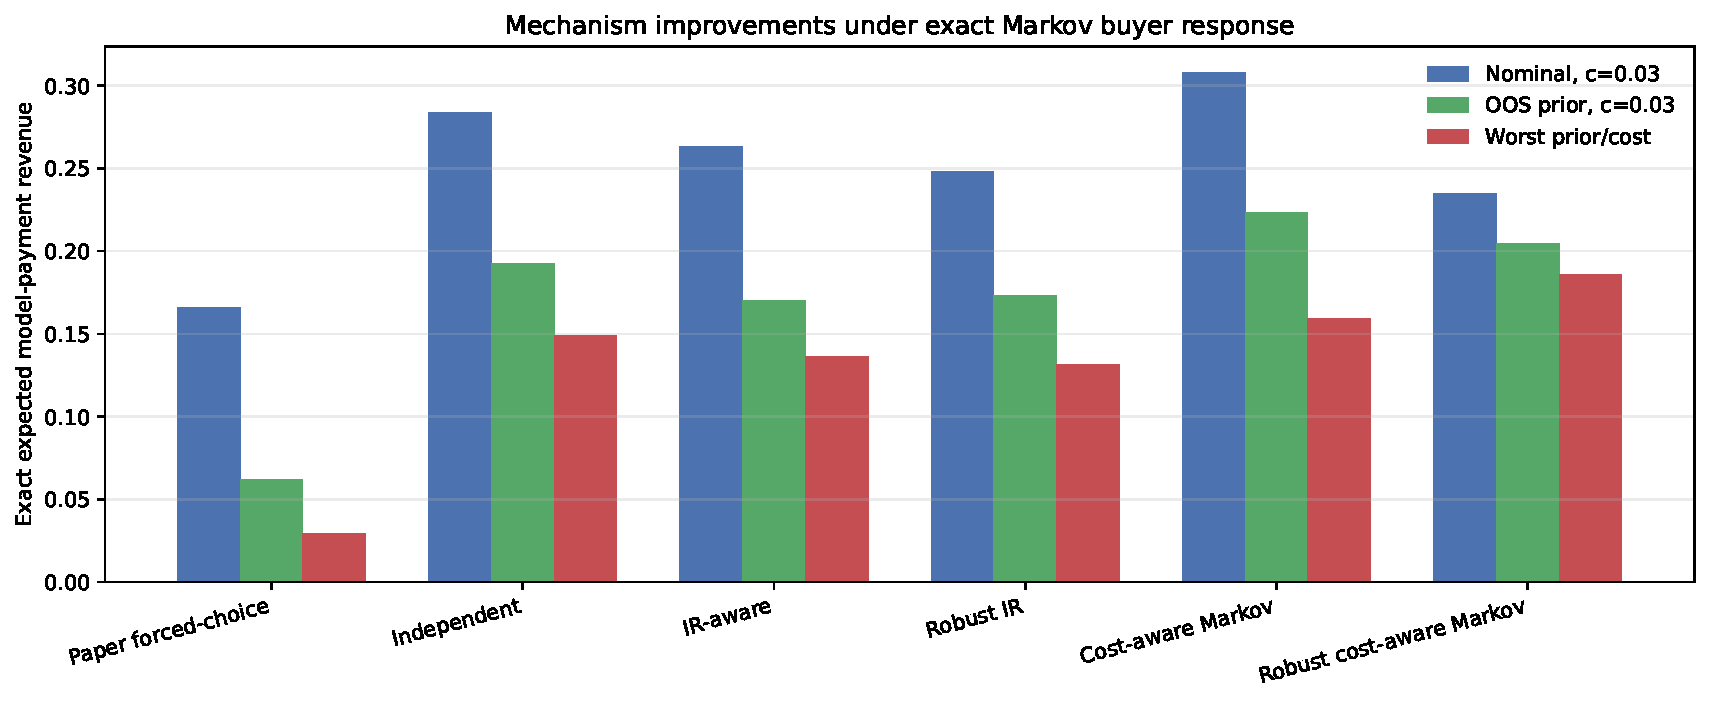
\includegraphics[width=0.94\textwidth]{improvement_pricing_revenue.pdf}
\caption{主实例：名义先验、OOS 先验和最坏先验/成本下的精确 Markov 收入。}
\end{figure}

\begin{table}[H]
\centering
\small
\caption{主实例的精确 Markov 收入。}
\begin{tabular}{lrrr}
\toprule
方法 & 名义 $c=0.03$ & OOS 先验 $c=0.03$ & 最坏先验/成本\\
\midrule
Paper forced-choice & 0.1658 & 0.0622 & 0.0296\\
Independent & 0.2838 & 0.1927 & 0.1490\\
IR-aware & 0.2634 & 0.1702 & 0.1366\\
Robust IR & 0.2478 & 0.1729 & 0.1317\\
Cost-aware Markov & \textbf{0.3082} & \textbf{0.2231} & 0.1592\\
Robust cost-aware Markov & 0.2347 & 0.2049 & \textbf{0.1857}\\
\bottomrule
\end{tabular}
\end{table}

\begin{resultbox}{主实例怎样解读}
\begin{itemize}
  \item Cost-aware Markov 相比 Independent 的名义收入提高约 8.6\%，OOS 先验收入提高约 15.8\%，说明搜索成本与停止顺序确实会改变最优价格。
  \item Robust cost-aware Markov 相比 Independent 的最坏情况收入提高约 24.6\%。
  \item 鲁棒方案的代价很明确：相对 Cost-aware Markov，其名义收入下降约 23.9\%。因此“鲁棒”不等于“所有指标都高”。
  \item IR-aware 的意义首先是口径正确；它在本主实例上没有支配 Independent。
\end{itemize}
\end{resultbox}

\begin{figure}[H]
\centering
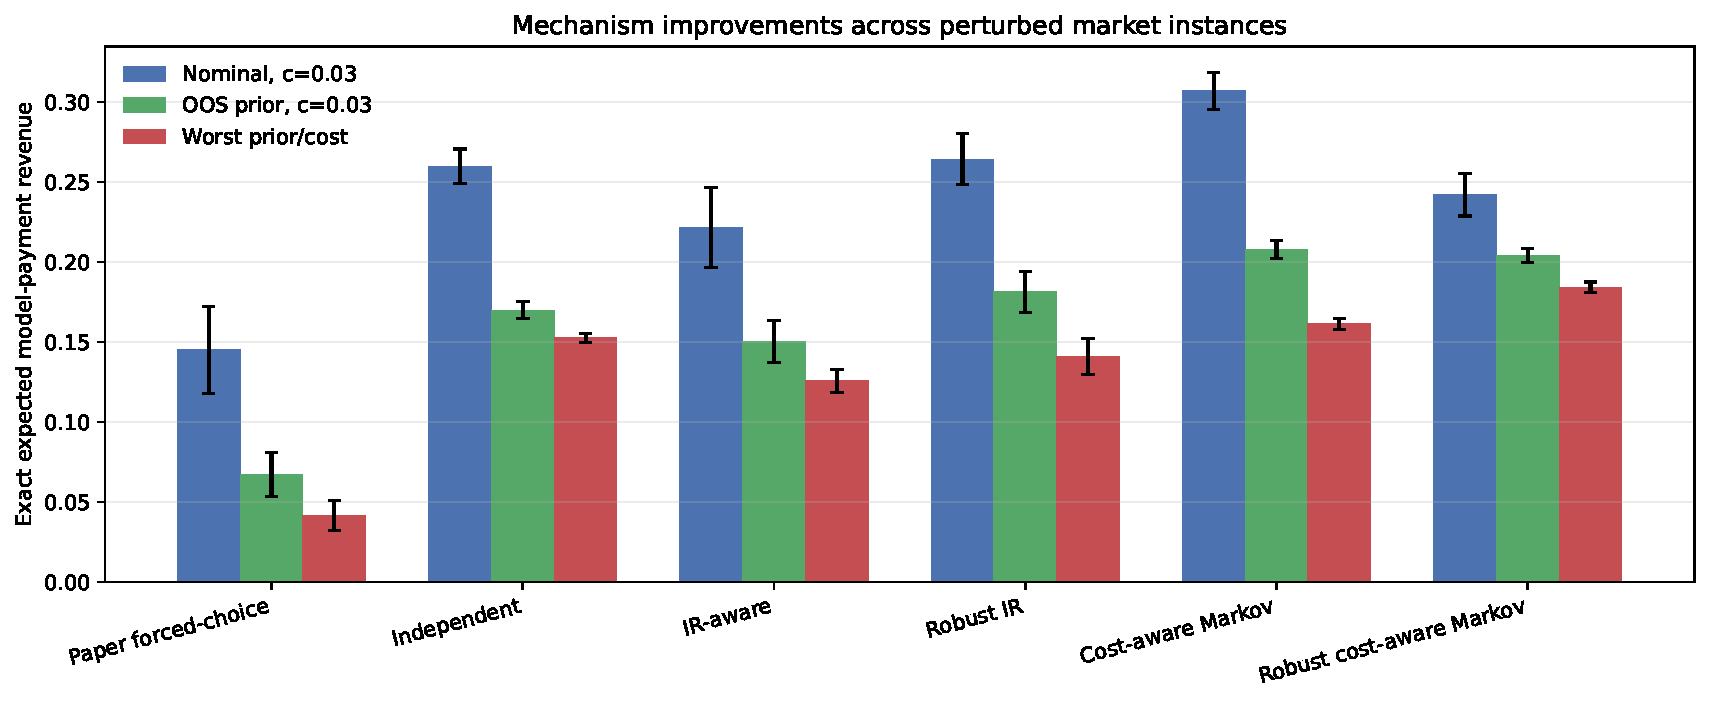
\includegraphics[width=0.94\textwidth]{improvement_pricing_multi_instance.pdf}
\caption{5 个扰动市场上的定价收入均值与标准误。}
\end{figure}

\begin{table}[H]
\centering
\small
\caption{5 个扰动市场的均值 $\pm$ 标准误。}
\begin{tabular}{lrrr}
\toprule
方法 & 名义 $c=0.03$ & OOS 先验 $c=0.03$ & 最坏先验/成本\\
\midrule
Paper forced-choice & $0.1451\pm0.0273$ & $0.0673\pm0.0137$ & $0.0417\pm0.0094$\\
Independent & $0.2600\pm0.0107$ & $0.1698\pm0.0053$ & $0.1527\pm0.0026$\\
IR-aware & $0.2217\pm0.0250$ & $0.1503\pm0.0131$ & $0.1257\pm0.0072$\\
Robust IR & $0.2644\pm0.0158$ & $0.1814\pm0.0130$ & $0.1411\pm0.0112$\\
Cost-aware Markov & $\mathbf{0.3072}\pm0.0116$ & $\mathbf{0.2079}\pm0.0056$ & $0.1614\pm0.0034$\\
Robust cost-aware Markov & $0.2420\pm0.0131$ & $0.2041\pm0.0045$ & $\mathbf{0.1843}\pm0.0033$\\
\bottomrule
\end{tabular}
\end{table}

多实例结果保持相同排序：名义市场偏向 Cost-aware Markov，最坏情况偏向 Robust cost-aware Markov。5 个实例仍然是小样本，因此标准误只能表示这组透明扰动下的稳定性，不能替代更大规模统计检验。

\section{实验结果：定价引导发现}

\begin{figure}[H]
\centering
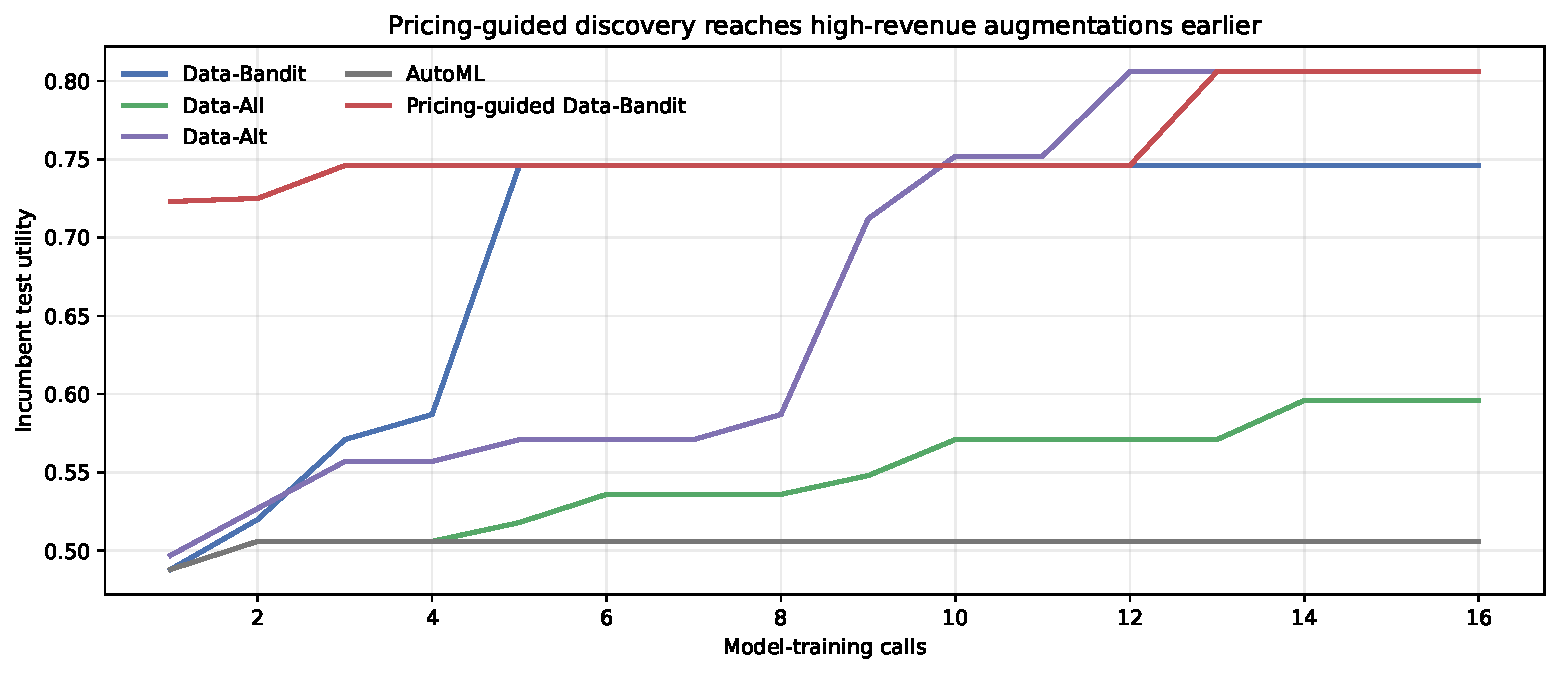
\includegraphics[width=0.92\textwidth]{improvement_discovery_curves.pdf}
\caption{主 score table：Pricing-guided Data-Bandit 更早进入高效用区域。}
\end{figure}

\begin{table}[H]
\centering
\small
\caption{主 score table 的发现结果，预算为 16。}
\begin{tabular}{lrrrr}
\toprule
方法 & 最终效用 & AUC & 95\% 训练数 & 前 4 次效用\\
\midrule
Data-Bandit & 0.7460 & 0.6949 & 17 & 0.5415\\
Data-All & 0.5960 & 0.5470 & 17 & 0.5015\\
Data-Alt & \textbf{0.8060} & 0.6678 & 12 & 0.5345\\
AutoML & 0.5060 & 0.5049 & 17 & 0.5015\\
Pricing-guided Data-Bandit & \textbf{0.8060} & \textbf{0.7583} & 13 & \textbf{0.7350}\\
\bottomrule
\end{tabular}
\end{table}

\begin{resultbox}{主发现实验怎样解读}
Pricing-guided Data-Bandit 相比普通 Data-Bandit 的 AUC 增加 0.0634，前 4 次训练平均效用提高约 35.7\%。它最终达到 0.8060，与 Data-Alt 并列最高。收益集中在“更早发现”，这正是 warm-start 信号应发挥作用的阶段。
\end{resultbox}

\begin{figure}[H]
\centering
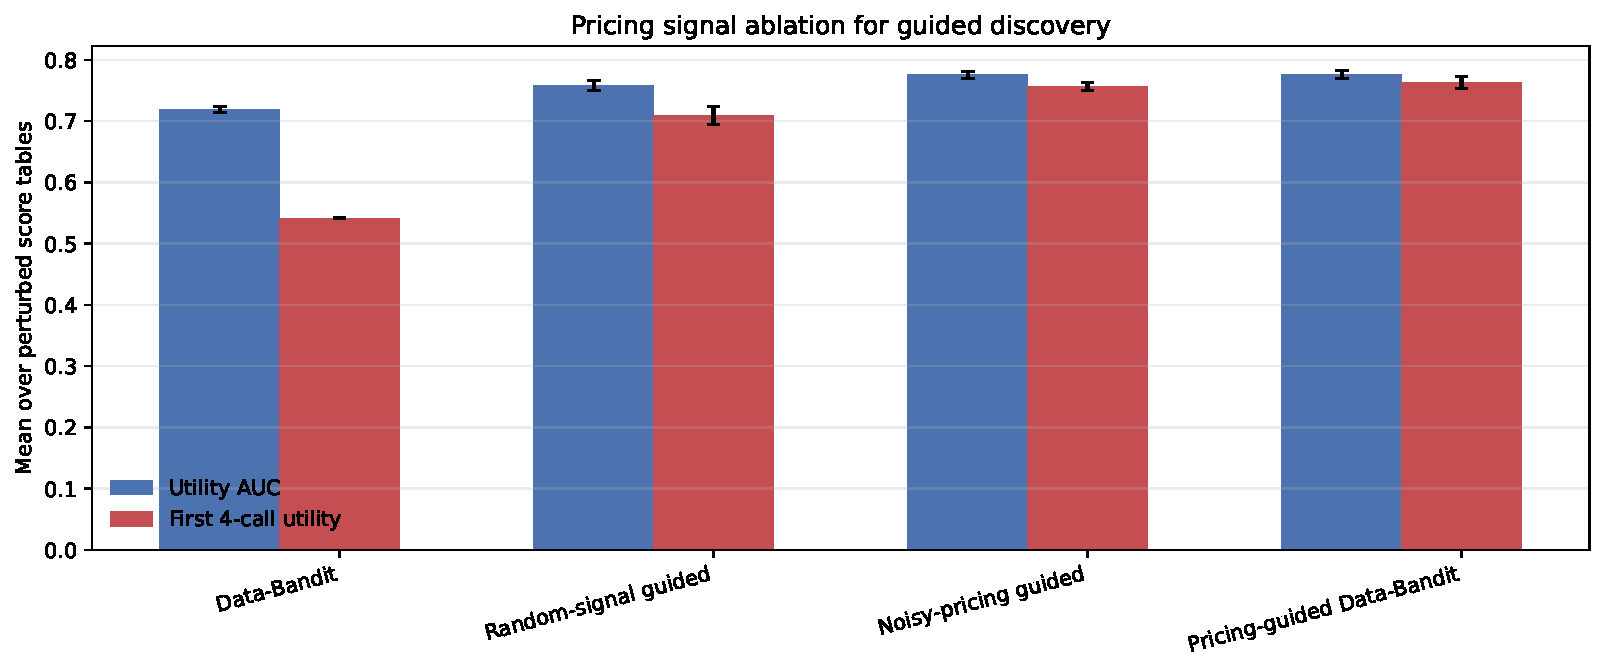
\includegraphics[width=0.92\textwidth]{improvement_discovery_signal_ablation.pdf}
\caption{12 个扰动 score table 上的价格信号消融。}
\end{figure}

\begin{table}[H]
\centering
\small
\caption{价格信号消融，均值 $\pm$ 标准误。}
\begin{tabular}{lrr}
\toprule
方法 & AUC & 前 4 次效用\\
\midrule
Data-Bandit & $0.7191\pm0.0042$ & $0.5418\pm0.0009$\\
Random-signal guided & $0.7588\pm0.0081$ & $0.7096\pm0.0147$\\
Noisy-pricing guided & $0.7756\pm0.0052$ & $0.7566\pm0.0071$\\
Pricing-guided Data-Bandit & $\mathbf{0.7764}\pm0.0070$ & $\mathbf{0.7630}\pm0.0094$\\
\bottomrule
\end{tabular}
\end{table}

随机信号本身已经比普通 Data-Bandit 高，说明“改变访问顺序并更早集中探索”贡献了相当一部分收益。真实价格信号相对随机信号的 AUC 增量约为 0.0176，且 Noisy-pricing 与真实信号接近。因此正确结论是：warm-start 价格信号在排序收益之外提供了\emph{有限增量}，而不是无条件显著优越。

\section{测试、复现命令与产物}

完整环境使用 \path{environment.yml}，其中固定 Python 主版本以及 NumPy、Matplotlib 和 HiGHS 版本。主要命令为：

\begin{lstlisting}[language=bash]
conda run -n automl-market make test
conda run -n automl-market make improvements
conda run -n automl-market make improvement-report
\end{lstlisting}

当前 20 项单元测试全部通过。与本报告直接相关的测试覆盖：

\begin{itemize}
  \item 外部选项能移除不可实现收入；
  \item 精确 Markov 支付遵循最优停止策略；
  \item 时间变化转移矩阵不会在终点越界；
  \item 鲁棒成本感知目标等于声明场景中的最坏收入；
  \item 价格信号会加入引导发现方法并优先高信号增强；
  \item 所有发现方法遵守模型训练预算。
\end{itemize}

数值依据位于：

\begin{itemize}
  \item \path{results/improvement_experiments_summary.json}；
  \item \path{results/tables/improvement_pricing_results.csv}；
  \item \path{results/tables/improvement_pricing_multi_instance.csv}；
  \item \path{results/tables/improvement_discovery_results.csv}；
  \item \path{results/tables/improvement_discovery_signal_ablation.csv}。
\end{itemize}

\section{结论与适用边界}

\begin{enumerate}
  \item \textbf{外部选项}让收入指标符合自愿购买语义，但不保证收入高于 Independent。
  \item \textbf{成本感知 Markov 定价}把价格、停止策略、质量顺序与搜索成本放入同一动态目标；对给定价格的收入是精确的，价格搜索仍是有限网格。
  \item \textbf{联合鲁棒定价}提高显式先验/成本场景中的收入下界，同时牺牲名义收入；它不是完整 DRO。
  \item \textbf{价格引导发现}在存在可用 warm-start 信号时改善早期发现效率；冷启动第一单和真实信号构造仍是开放问题。
\end{enumerate}

四项改进共同把原论文的理想化机制推进到更可部署的方向，但没有改变其核心价值主张：平台仍然对数据增强带来的可测模型性能提升收费，而不是按原始数据数量或训练计算量收费。现有实验构成了代码、测试、主实例、多实例、消融、表格和图像的闭环；下一步若继续研究，应优先扩展真实价格信号构造、更多市场实例、连续价格动态优化和严格分布鲁棒理论。

\begin{thebibliography}{9}
\bibitem{han2023}
Y. Han, S. Padmanabha, S. Wang, Z. Huang, and J. Zhao.
\newblock Optimal Pricing for Data-Augmented AutoML Marketplaces.
\newblock arXiv preprint arXiv:2310.17843, 2023.
\end{thebibliography}

\end{document}
